\documentclass{article}
\usepackage[utf8]{inputenc}
\usepackage[a4paper, portrait, margin=1in]{geometry}
\usepackage{tabularx}
\usepackage{graphicx}
\usepackage{amsmath}

\title{OOAD \& Software Engineering (UE18CS353) \\
    Unit 1}
\author{Aronya Baksy \and Vishnu Dixit}
\date{January 2021}

\begin{document}

\maketitle

\section{Introduction}
\begin{itemize}
    \item Software engineering is the application of a systematic, disciplined and quantifiable approach to the development, operation and maintenance of software. (\textit{defn. acc to NATO conference of 1968})
    
    \item Software engineering is the establishment and use of sound engineering principles in order to obtain economically, software that is reliable and works on real machines. (\textit{defn. acc to IEEE Standard Glossary}). 
\end{itemize}

\subsection{Characteristics of Software Engineering}
\begin{itemize}
    \item \textit{Concerns the development of large programs}: No clear distinction between large and small projects, but generally refers to multi-person and long-term development work of any software that consists of many interconnected components. 
    
    \item \textit{Mastering complexity is the central theme}: Complexity of software projects are generally due to vast number of details to be handled. Thus projects are split into smaller units (modules, components etc.) and each component is handled separately. 
    
    \item \textit{Software Evolves}: Evolution of software along with changing reality is a cost that has to be factored in during development. 
    
    \item \textit{Efficiency of SE is crucial}: Minimization of costs (labour, infra,  time etc.) associated with software development is important, thus giving rise to efficient methods of development and maintenance (useful: tools/methods that allow reuse of components). 
    
    \item \textit{Co-operation between people}: Clear arrangements for work distribution, communication and responsibilities etc. Standards and procedures are used to enforce these arrangements and ensure discipline. 
    
    \item \textit{Effective user support}: Identify functional requirements, address usability, reliability, responsiveness, user-friendliness. Also documentation and manuals for creating the right envt for software to function. 
    
    \item \textit{Balancing act}: between initial requirements (which may not be static) and the resources available to the developer (in terms of expertise) 
\end{itemize}

\section{Phases of Software Engineering (SDLC)}
\begin{itemize}
    \item The Software Development Life Cycle (SDLC) consists roughly of the following phases: \textbf{requirements engineering}, \textbf{design}, \textbf{implementation}, \textbf{testing} and \textbf{maintenance}. 
\end{itemize}

\subsection{Requirements Engineering}
\begin{itemize}
    \item Goal: get a complete description of the problem statement and the requirements posed by and on the functional environment of the software. 
    
    \item Important sub-phase here is feasibility study, which assesses the technical and economic feasibility of the solution to this problem. 
    
    \item Problem statement description may include the following:
    \begin{itemize}
        \item Functions of the software
        
        \item Possible future extensions
        
        \item Amount and kind of documentation needed
        
        \item Performance requirements and constraints (eg: max response time)
    \end{itemize}
    
    \item The output of this phase is a document called the \textbf{requirement specification}. 
\end{itemize}

\subsection{Design}
\begin{itemize}
    \item Creation of a model that aims to solve the problem.
    
    \item The first part of the design phase is \textit{interface design} wherein the interaction between the software and its environment is described. 
    
    \item The second part of design phase involves \textit{architectural design}, wherein a global high-level description of the system is created. This involves the component breakdown, roles/responsibilities of each component, properties of each component and interfaces between components. 
    
    \item The \textit{detailed design} is the further decomposition of components into program units which are allocated some functional responsibility. Data structures and algorithms, data communication between components, state definitions and change of state properties etc. are all dealt with here. 
    
    \item Output of the design phase is the \textbf{technical specification}
\end{itemize}

\subsection{Implementation}
\begin{itemize}
    \item Direct translation between specification to code, or might include an additional phase of translation to high-level \textit{pseudocode} first.
    
    \item Goal is to produce well-documented, reliable, easy-to-read, flexible and correct program. Emphasis over these as against efficiency using fancy optimizations.
    
    \item The overall structure that was created in the design phase might get lost in translation to programming. More modern languages allow one to retain this structure to a large extent. 
    
    \item The output of this phase is an executable program. 
\end{itemize}

\subsection{Testing}
\begin{itemize}
    \item Testing most often does not follow implementation phase, rather it happens in parallel with implementation. 
    
    \item \textbf{Verification}: Testing whether the transition between phase boundaries in the SD process is valid or not.
    
    \item \textbf{Validation}: Checking whether the current status of the software is in keeping with the user requirements specified in the requirement engineering phase. 
    
    \item The output of this phase is the tested executable program. 
\end{itemize}

\subsection{Maintenance}
\begin{itemize}
    \item Activities that keep system operational after delivery to the user. 
    
    \item This involves changes/enhancements to the user requirements post delivery, as well as correction of any errors that are not detected in the testing phase. 
\end{itemize}

As per the \textit{40-20-40 rule} 40\% of effort is used up in the requirement engineering and design phases, 20\% for implementation and 40\% for testing. 


\section{Development Life Cycles}
\subsection{Software Development Life Cycle}
\begin{itemize}
    \item SDLC is a structured set of activities in a fixed order, generating intermediate and final results.
    
    \item Each activity (step) has a guiding principle that explains its end goal 
    
    \item A product is the outcome of applying a process (i.e. this sequence of steps) on a project.
    
    \item Each phase has the following:
    \begin{enumerate}
        \item Entry criteria
        \item Exit criteria
        \item Task to be done
        \item Person responsible
        \item Dependencies
        \item Constraints (scheduling, etc.)
    \end{enumerate}
\end{itemize}

\subsection{Product Development Life Cycle}
\begin{itemize}
    \item A process that is responsible for bringing to market a new product and generally includes the business units.
    
    \item SDLC is more pointed towards solving software-specific problems. Hence SDLC is a subset of the PDLC, and the SDLC points to specific steps within the PDLC.
    
    \item A generic PDLC consists of the following phases:
    \begin{enumerate}
        \item \textbf{Planning}: Involves requirement, scope gathering 
        
        \item \textbf{Analysis}: Involves research and usability engineering
        
        \item \textbf{Design}
        
        \item \textbf{Implementation}
        
        \item \textbf{Testing and Quality Assurance (QA)}
        
        \item \textbf{Deployment }
        
        \item \textbf{Training and sales support}
        
        \item \textbf{Maintenance and technical support}
    \end{enumerate}
\end{itemize}

\subsection{Project Management Life Cycle}
\label{pmlc}
\begin{itemize}
    \item A high level description of processes involved in delivering a successful project. 
    
    \item The PMLC consists of the following phases:
    \begin{enumerate}
        \item \textbf{Initiation}: Involves developing a business case, identifying scope and stakeholders 
        
        \item \textbf{Planning}: Workflow plan, budget plan, gather resources
        
        \item \textbf{Execution, Direction and Control}: Involves requirement engg, design, implementation and testing 
        
        \item \textbf{Closure}: Project review (goals met or not), team review (team's performance), documentation, process improvement for future projects
    \end{enumerate}
\end{itemize}

\subsection{Software Maintenance Life Cycle}
\begin{itemize}
    \item Structured process of implementing any changes to a delivered software. 
    
    \item The SMLC is triggered by a change request from the client. 
    
    \item After a change request is received, the steps in the SMLC are:
    \begin{itemize}
        \item \textbf{Problem Identification}: Assign a unique number to the issue, add it to repository and accept/reject the request after validation.
        
        \item \textbf{Analysis}: Technical review, feasibility study, identify potential side effects (security, performance etc.)
        
        \item \textbf{Design}: Revise design, develop test cases, verify the revised design
        
        \item \textbf{Implementation}: Implement revised design, review software, unit test
        
        \item \textbf{System Testing}: System, acceptance and regression testing
        
        \item \textbf{Delivery} 
    \end{itemize}
\end{itemize}

\subsection{Product Life Cycle}
\begin{itemize}
    \item The phases of a product from the time it is introduced to consumers into the market until it is removed from the shelves.
    
    \item The phases of  PLC are:
    \begin{itemize}
        \item \textbf{Introduction}: Invest in marketing and advertisement
        
        \item \textbf{Growth}: Growing demand, ramp up production, expand availability of the product
        
        \item \textbf{Maturity}: Most profitable stage, marketing and production costs decline
        
        \item \textbf{Decline}: Increased competition leads to reduced market share and decline in profits.
    \end{itemize}
\end{itemize}

\section{Legacy SDLC Models}

\subsection{Waterfall Model}
\begin{itemize}
    \item In figure \ref{fig:my_label}, V\&V stands for \textit{Verification} and \textit{Validation}.
    
    \item Before moving on to the next stage of the waterfall model, the previous stage undergoes both Verification (whether the software meets its own requirements) and Validation (whether the software meets the user requirements). 
\end{itemize}

\subsubsection{Use case of Waterfall Model}
The waterfall model is suitable when:
\begin{itemize}
    \item Requirements are clear, well-documented, fixed and unambiguous
    
    \item Definition of product is stable
    
    \item Technology is well understood, ample resources are available to support 
    
    \item Project is short
\end{itemize}

\begin{figure}[!h]
    \centering
    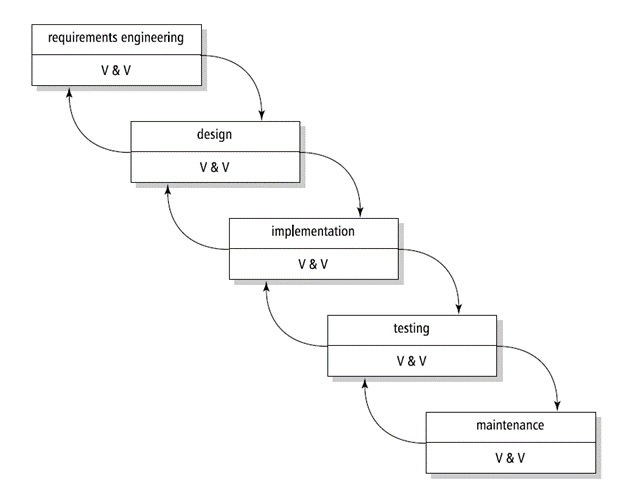
\includegraphics[scale=0.5]{se1.png}
    \caption{Waterfall Model}
    \label{fig:my_label}
\end{figure}

\subsubsection{Advantages}
\begin{itemize}
    \item Simple to understand and use, with well defined phases and milestones for each stage.
    
    \item Process and results are well documented. 
    
    \item Easy to manage due to the inherent rigidity of the model.
    
    \item Each phase has specific deliverables and review process. 
\end{itemize}

\subsubsection{Disadvantages}
\begin{itemize}
    \item No working software is produced until late in the development cycle. 
    
    \item High risk and uncertainty due to the rigidity of the model. This makes it hard to accommodate changing requirements and scope. 
    
    \item Poor choice for long, complex, object-oriented projects 
    
    \item Difficult to measure progress within stages
    
    \item Integration is done only at the end (in a big-bang manner), hence it is hard to identify technical or business challenges/bottlenecks early. 
\end{itemize}

\subsection{V Model}
\begin{itemize}
    \item For each phase in the development pipeline, there is a corresponding test phase. The corresponding development and test phases are \textit{planned} (ie. designed) in parallel.
    
    \item The left side of the V indicates the Verification phases and the right side indicates the Validation phases.
    
    \item Verification phases:
    \begin{itemize}
        \item \textbf{Requirement Analysis}: Get requirements from customer
        
        \item \textbf{System Design}: Component design, communication and hardware setup for system
        
        \item \textbf{Architectural Design}: Break down into modules, functionalities of each module as well as inter- and intra-module communication is detailed. 
        
        \item \textbf{Module Design}: Low level Design (LLD) of modules is specified here
    \end{itemize}
    
    \item Validation Phases
    \begin{itemize}
        \item \textbf{Unit Testing}: Elimination of bugs at the unit level or code level
        
        \item \textbf{Integration Testing}: Verify communication of modules with each other
        
        \item \textbf{System Testing}: Functionalities of the complete software along with all inter-dependencies and communication is tested here. Tests functional and non-functional requirements
        
        \item \textbf{Acceptance Testing}: This is done in a real-life environment that resembles the actual production environment. This verifies that the system meets the requirements and is suitable for real-world use. 
    \end{itemize}
\end{itemize}

\begin{figure}[!h]
    \centering
    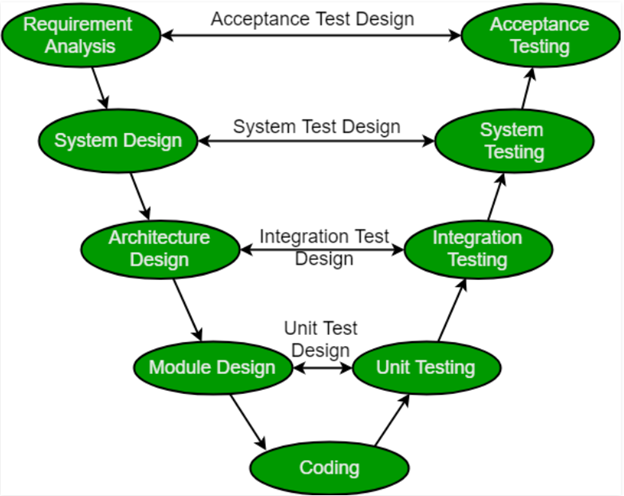
\includegraphics[scale=0.7]{se2.png}
    \caption{V Model}
    \label{fig:my_label_2}
\end{figure}

\subsubsection{Advantages}
\begin{itemize}
    \item Focus on verification and validation activities early on in life cycle leads to error-free and better quality final product. 
    
    \item More accurate progress tracking by project management
    
    \item Highly disciplined model with sequential phases 
\end{itemize}

\subsubsection{Disadvantages}
\begin{itemize}
    \item High risk and uncertainty, not suitable for dynamic user requirements
    
    \item Does not support iteration of phases, does not handle concurrent events
    
    \item Not good for object-oriented and complex projects
    
    \item No code is generated until the implementation phase hence no early prototypes are produced. 
    
    \item Changes in verification stage need to be mirrored in the validation (testing) phase which leads to duplication of effort. 
\end{itemize}

\subsection{Prototyping Model}
\begin{itemize}
    \item This model is used when customer requirements are not well defined initially. 
    
    \item A prototype (ie. an initial basic model of the system) is built and refined iteratively as per customer feedback until an acceptable prototype is built. This serves as the basis for the final software product. 
    
    \item Types of prototyping activities:
    \begin{itemize}
        \item \textbf{Rapid Throwaway Prototyping}: In this method, a developed prototype need not necessarily be a part of the ultimately accepted prototype. Customer feedback helps in preventing unnecessary design faults.
        
        \item \textbf{Evolutionary Prototyping}: The initial prototype is incrementally modified on the basis of customer feedback until an accepted prototype is created. This saves time and effort in comparison to throwaway prototyping. 
        
        \item \textbf{Incremental Prototyping}: The project is initially broken up into components, each component is prototyped individually and all components are integrated at the end. Leads to substantial cost saving but proper communication has to be ensured so that modules integrate properly at the end. 
        
        \item \textbf{Extreme Prototyping}: Used in website design typically. Consists of 3 stages \begin{enumerate}
            \item Basic prototype with existing static pages (wireframe) 
            
            \item Functional screens that simulate a data process using a prototype service layer
            
            \item All services implemented and associated with final prototype
        \end{enumerate}
    \end{itemize}
\end{itemize}

\subsubsection{Advantages}
\begin{itemize}
    \item Code is generated early in the life cycle, meaning more opportunities to get customer feedback and refine the system.
    
    \item Easy to accommodate new requirements and add new features/missing features. 
    
    \item Early error detection that reduces costs and effort, while improving software quality
    
    \item Prototypes once built can be reused for future projects
\end{itemize}

\subsubsection{Disadvantages}
\begin{itemize}
    \item Costly wrt time and money, especially if user requirements vary a lot. 
    
    \item Documentation suffers due to constantly changing requirements.
    
    \item Leads to increasing complexity if changes suggested exceed the original scope of the project. 
    
    \item Performance of the resulting system may not be optimal
\end{itemize}
\begin{figure}[!ht]
    \centering
    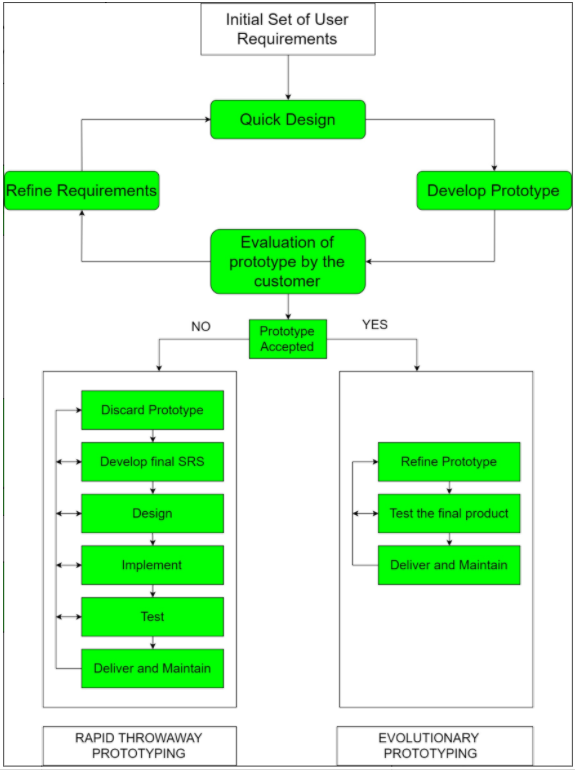
\includegraphics[scale=0.5]{se3.png}
    \caption{Prototyping Model}
    \label{fig:my_label_3}
\end{figure}

\subsection{Incremental Model}
\begin{itemize}
    \item The functionality of the system is produced and delivered to the customer in small increments. 
    
    \item Each subsequent release of the project adds a new functionality to the previous release. 
    \item The 'Big Bang' effect is avoided in this approach as software is developed in a phased manner module by module, hence leading to more flexibility in terms of changing requirements.
    
    \item The process of development is split into partitions, where each partition corresponds to one release of the software. Each partition is planned using a model like the Waterfall model.
\end{itemize}

\subsubsection{Advantages}
\begin{itemize}
    \item Early delivery to customer means greater value to customer. 
    
    \item More flexible, less costly to change requirements and scope of project. 
    
    \item Easy to manage risk, by handling the most risky components in conjunction with customer feedback. 
    
    \item Reduces over-functionality, incremental model leads to development of essential modules first and additional modules later.
\end{itemize}

\subsubsection{Disadvantages}
\begin{itemize}
    \item Good planning and design, needs complete and comprehensive definition of project before splitting into increments. 
    
    \item Higher cost than equivalent waterfall model. 
    
    \item Hard to identify facilities common to each increment. 
    
    \item Management visibility is reduced which could lead to surprises
\end{itemize}

\subsection{Iterative Model}
\begin{itemize}
    \item Initially a skeleton implementation, is refined with user feedback and iterative evolution to give a complete system. 
    
    \item Dummy modules substitute for incomplete components,
    
    \item Rapid prototyping and successive refinement are the driving principles
\end{itemize}

\subsubsection{Advantages}
\begin{itemize}
    \item Early visualization of solution
    
    \item Risk mitigation supported
    
    \item Effects of a defect flowing down the life cycle is reduced
    
    \item Incremental investment
\end{itemize}

\subsubsection{Disadvantages}
\begin{itemize}
    \item Rigid with overlaps 
    
    \item Costly system architecture or design issues may arise because not all requirements are gathered up front for the entire life cycle
\end{itemize}

\subsection{Limitations of legacy models}
\begin{itemize}
    \item Require predictive development methods, upfront planning
    
    \item Suitable only for projects where requirements don't change often, and are well understood at the start
    
    \item Do not facilitate regular interaction with client 
\end{itemize}

\section{Agile and SCRUM}
\subsection{Agile}
\begin{itemize}
    \item Agile practices involve discovering requirements and developing solutions through the \textbf{collaborative effort} of \textbf{self-organizing} and \textbf{cross-functional} teams and their clients. 
    
    \item Aims:
    \begin{itemize}
    
        \item Deliver value to client as quickly as possible
        
        \item Allow continuous realignment of development goals with customer needs
        
        \item Reduce planning overheads
    \end{itemize}
\end{itemize}

\subsubsection{Advantages of Agile methodologies}
\begin{itemize}
    \item Rapid development and demonstration of functionalities, delivers partially working solutions faster (concurrent delivery and development in a planned context)
    
    \item Works when client's requirements are dynamic
    
    \item Minimal resource and planning requirements, easy to manage
    
    \item Promote teamwork, cross-training, flexibility to developers
\end{itemize}

\subsubsection{Drawbacks of Agile methodologies}
\begin{itemize}
    \item Not suitable for complex dependencies
    
    \item Driven by client requirements, if client is not clear then team works in wrong direction
    
    \item Sustainability, maintainability and extensibility are more risky to implement
    
    \item Minimum documentation leads to high individual dependency and high cost of knowledge transfer. 
\end{itemize}

\subsection{Scrum}
\begin{itemize}
    \item Scrum is an Agile framework for developing, delivering and maintaining software products. It is an \textit{iterative} approach
    
    \item Key ideas of Scrum:
    \begin{enumerate}
        \item Iterative and incremental approach, encourages physical or close online collaboration of team members 
        
        \item Requirements are not static
        
        \item Maximize the team's ability to deliver quickly, and adapt to technological change, competition and changing requirements.
    \end{enumerate}
\end{itemize}

\subsubsection{Scrum Roles}
\begin{itemize}
    \item \textbf{Product Owner}: Represents the customer and the stakeholders,and is responsible for delivering business results.  
    
    \item The product owner defines the product in terms of user stories, adds them to the Product Backlog, and prioritizes them based on importance and dependencies.
    
    \item \textbf{Scrum Master}: Not a traditional team lead or manager, instead focus on removing obstacles towards successful goal delivery. 
    
    \item Scrum Master ensures that Scrum principles are followed, and facilitates team meetings.
    
    \item \textbf{Developer}: build increments of valuable work after every sprint. Can be anyone involved in R\&D, statisticians, programmers and testers. 
    
    \item Developers are also referred to as scrum team members. A team of developers is self-organized and cross-functional.
\end{itemize}

\subsubsection{Scrum Artifacts}
\begin{itemize}
    \item The \textbf{product backlog} is a description of the product in the form of features told from the user's perspective (user stories)
    
    \item The scrum team estimates the work associated with each story and ranks them in the order of importance
    
    \item The weighted-ranked features/stories in the backlog results in \textbf{roadmap} 
    
    \item The features/stories in the backlog planned for a sprint is the \textbf{sprint backlog}
\end{itemize}

\subsubsection{Scrum Events}
\begin{itemize}
    \item The \textbf{Split} is the basic unit of development time. Commonly kept at 2 weeks, it is a \textit{sandboxed} effort (the time is pre-planned and fixed).
    
    \item \textbf{Sprint Planning} involves deciding the scope of a sprint, prepare a sprint goal and a sprint backlog. 
    
    \item A \textbf{Daily Scrum} meeting involves discussing work done yesterday, work to be done today and obstacles to achieving the sprint goal. 
    
    \item A \textbf{Sprint Review} is held at the end of each sprint. It involves reviewing work done and not done as planned in the sprint, a \textit{demo} of the completed work and collaborating with stakeholders on what to work on next. 
    
    \item A \textbf{Sprint Retrospective} is also held at the end of each sprint. The team reflects on the past sprint, identifies and agrees on continuous process improvement actions
    
    \item The retrospective is attended by the Scrum master.
\end{itemize}

\section{Component-Based Software Engineering}
\subsection{CBSE}
\begin{itemize}
    \item A reuse-based approach to define, implement or select off-the-shelf components and integrate these loosely-coupled components into functioning systems. 
    
    \item Essential properties of CBSE are:
    \begin{itemize}
        \item Independent components that are completely specified by the public interfaces 
        
        \item Component standards that facilitate integration
        
        \item Middleware that provides support for integration
        
        \item Development process geared towards CBSE
    \end{itemize}
    
    \item A component is an independent executable entity that implements a functionality while hiding its implementation details.
    
    \item All interactions with the component are made via the published interface. 
    
    \item Required dependencies and published interfaces are indicated as part of a component. 
    
    \item Component selection involves:
    \begin{itemize}
        \item Select existing components after searching
        
        \item Compose existing components using direct connection or adapters for different interfaces. 
        
        \item Validation
    \end{itemize}
    
    \item Specification describes properties to be realized: realization contract,  Interface describes how components interact: usage contract

    
    \item CBSE model consists of the following:
    \begin{itemize}
        \item Interfaces: defines interaction, and names, parameters, exceptions to be included in the interface definition
        
        \item 
    \end{itemize}
    
    \item Advantages of CBSE:
    \begin{itemize}
        \item Reduces complexity of systems as components are black boxes
        
        \item Reduced development time due to reuse, increased productivity.
        
        \item Increase in quality, maintainability (explicit dependencies, reuse)
    \end{itemize}
    
    \item Drawbacks of CBSE:
    \begin{itemize}
        \item Component trustworthiness, certification
        
        \item Requirement trade-off
        
        \item Emergent property prediction
    \end{itemize}
\end{itemize}

\subsection{Service-Oriented Architecture}
\begin{itemize}
    \item Structured collections of software modules, known as services, that collectively provide the complete functionality of a large application. 
    
    \item Consists of:
    \begin{itemize}
        \item \textbf{Infrastructure Service Layer}: Supporting activities such as data storage, databases etc.
        
        \item \textbf{Business Service Layer}: Business logic modules deployed in the form of individual containers
        
        \item \textbf{Orchestration Layer}: Manages and co-ordinates the containers deployed.
        
        \item \textbf{System Bus} for communication between layers
    \end{itemize}
\end{itemize}

\subsection{Product Lines}
\begin{itemize}
    \item Software product lines refers to techniques for creating a collection of similar software systems from a shared set of software assets
    
    \item A top-down, planned, proactive approach to achieve reuse of software within a family of products. 
    
    \item Exploits commonality and variability between requirements of different product lines, for increased customization.
\end{itemize}
\subsubsection{Key Drivers}
\begin{itemize}
    \item Predictive rather than opportunistic (ad-hoc) reuse
    
    \item Artifacts are created when reuse is predicted in one or more products in a well defined product line
    
    \item These artifacts are either reusable components or design patterns that compose multiple components for a particular solution.
\end{itemize}

\section{Requirement Analysis}
\begin{itemize}
    \item The first step of any software project. The most error-prone and costly stage of the project. 
    
    \item Errors in this phase propagate and are hard to fix in later stages. 
    
    \item Requirement is the property which must be exhibited by software to solve a particular problem (more focus on what and not how)
\end{itemize}

\subsection{Properties of a requirement}
\begin{itemize}
    \item \textbf{Clear}: Precise, simple language, with active present tense, consistent terminology and keep requirements separate
    
    \item \textbf{Concise}: Explain only one property in fewest possible words
    
    \item \textbf{Consistent}: Requirements should not contradict one another
    
    \item \textbf{Unambiguous}: Only one interpretation
    
    \item \textbf{Feasible}: Can be realized within a specific timeframe
    
    \item \textbf{Traceable}: Back to client request, and forward to the software interface
    
    \item \textbf{Verifiable}: Has a testable criterion and a cost-effective to verify that it has been achieved
    
    \item \textbf{Quantizable}: Can be quantized, easier to verify
    
    \item \textbf{Prioritized}: Each requirement has a priority
\end{itemize}

\subsection{Feasibility Study}
\begin{itemize}
    \item In discussion with the clients
    
    \item Identify current solution, target customer, future market place
    
    \item Potential benefits
    
    \item A high level scope and understanding of the solution
    
    \item Technological, marketing and financial considerations
    
    \item Issues, Assumptions, Risks and Constraints
    
    \item High level planning and budget requirements, project organization
    
    \item Alternatives and their consideration
    
    \item The end result is a go/no go decision

\end{itemize}

\subsection{Steps in Requirement Engineering}
\subsubsection{Elicitation}
\begin{itemize}
    \item Gathering needs of stakeholders, communicating their problems.
    
    \item Establish clear scope and boundary for project.
    
    \item Understand the domain, the problem, the user needs, constraints. Identify the business objectives
    
    \item \textbf{Active Elicitation}: Ongoing and frequent interaction between client and stakeholders. Involves the use of interviews, prototyping, role-playing, scenarios and ethnography
    
    \item \textbf{Passive Elicitation}: Infrequent interaction between users and stakeholders. Involves the use of use cases, workflows, documentation, checklists, questionnaires, business process analysis
\end{itemize}

\subsubsection{Analysis}
\begin{itemize}
    \item Understand requirements from product and process perspective
    
    \item Classify requirements into coherent clusters, as functional/non-functional/domain requirements and system/user requirements
    
    \item Model the requirements (informal: prose, formal: flowchart, pseudocode, ER Diagram, dynamic models, UML based use-case diagram)
    
    \item Analyze requirements using fish-bone diagram (cause-effect)
    
    \item Recognize and resolve conflict (functionality vs timeline vs cost)
    
    \item Negotiate requirements, prioritize them using MoSCoW rule (\textbf{M}ust Have, \textbf{S}hould have, \textbf{Co}uld have, \textbf{W}on't have)
    
    \item Identify risks
    
    \item Decide to build or buy (COTS) and refine requirements
\end{itemize}

\subsubsection{Specification}
\begin{itemize}
    \item Document the requirements and give direction to the rest of the phases in the development life cycle.
    
    \item The SRS (Software Requirement Specification) is the basis for customers and suppliers agreeing on what the product will and won't do. It describes both the functional and nonfunctional requirements
    
    \item Documentation leads to more clarity, visibility, maintenance and evolution, team communication
    
    \item Document must be accurate, up-to-date, maintained online, simple and professional in appearance
    
    \item The SRS defines:
    \begin{itemize}
        \item \textbf{Functional Requirements}: Exact functionalities of the system
        
        \item \textbf{Non-functional Requirements}: All quality criteria that drive the functionality, such as performance (response/recovery time), availability, portability etc.
        
        \item \textbf{External Interfaces}: Interaction of the software with external hardware, software and people
        
        \item \textbf{Design Constraints}: Implementation language, standards and guidelines, resource limits, database integrity constraints, security and operating envt. etc. 
    \end{itemize}
    
    \item The \textbf{IEEE 830} template (1998) is a widely-accepted SRS template. 
\end{itemize}

\subsubsection{Validation}
\begin{itemize}
    \item Essential because repairing requirements in later phases is very expensive.

    
    \item Verification: Determines whether the requirement is specified correctly. 
    
    \item Review: for correctness, completeness, verifiability, traceability, and consistency.
    
    \item Prototyping: allows engineers and users to be involved in requirement engineering process, useful mostly for systems with high level of user interaction
    
    \item Validation: determines whether the user needs are satisfied by the requirement and whether the right problem is solved
    
    \item Usage of the Fish Bone Analysis technique to validate if the requirements identified is addressing the reasons needing the solution to the problem which had led to the requirements
    
    \item Acceptance Testing
\end{itemize}

\subsubsection{Requirement Management}
\begin{itemize}
    \item Ensure that all requirements are handled at each phase of SDLC, and requirement changes are handled appropriately.
    
    \item The Requirement Traceability Matrix (RTM) is filled out at each stage of the SDLC, and allows for forward and backward tracing of requirements.
\end{itemize}

\subsubsection{Change Management Process}
\begin{itemize}
    \item \textbf{Log} the change request (who, why, what to change), assign a change request identifier. 
    
    \item \textbf{Impact analysis} on schedule, quality, effort
    
    \item Solicit \textbf{Formal approval} from customer
    
    \item \textbf{Log} what changes were made, who made changes, when they were made, who reviewed and who tested changes, and the release stream that contains this change. 
\end{itemize}

\section{Project Management}
\begin{itemize}
    \item Planning and control of large projects that involve lots of people working over long time periods
    
    \item Characteristics of software project:
    \begin{enumerate}
        \item Consist of a sequence of unique activities that do not repeat and are inter-related to each other
        
        \item Goal-oriented
        
        \item Time-bound
    \end{enumerate}
    
    \item Project Management aims to maintain an equilibrium between cost, time and scope of the project.
    
    \item Refer to section \ref{pmlc} 
\end{itemize}
\subsection{Project Planning}
\begin{itemize}
    \item Focus on what to be implemented, how, make provisions for resources that may be required in the future.
    
    \item Project plan depends on the type of project (development, research etc.). It is an evolutionary document that changes with goals achieved, risks encountered, change in context or unforseen circumstances.
    
    \item Project Plan answers the questions:
    \begin{itemize}
        \item \textbf{Sponsor's POV}:
        \begin{itemize}
            \item Where does the product fit in with the roadmap of our organization
            
            \item Investment and revenue
            
            \item Time needed, resources needed, risks involved
            
            \item Deliverables and exit criteria
            
            \item Who is responsible, how is progress tracked
        \end{itemize}
        
        \item \textbf{Customer Perspective}: 
        \begin{itemize}
            \item Does the team understand the problem
            
            \item Time and cost needed
            
            \item Exit criteria
        \end{itemize}
        
        \item \textbf{Executor's Perspective}:
        \begin{itemize}
            \item Life cycle to follow
            
            \item How to prioritize the requirements
            
            \item Project organization (upstream/downstream relationships with other parts of the company, roles, user involvement)
            
            \item Standards, guidelines, comm mechanisms
            
            \item Schedule with detailed work breakdown and ownership
        \end{itemize}
    \end{itemize}
\end{itemize}

\subsubsection{Steps in project planning}
\begin{enumerate}
    \item Understand the deliverables: customer expectations, market forces behind the project, high level decisions of make-buy-reuse (based on the feasiblity study)
    
    \item Process plan: choose life cycle (based on goals, boundaries, time constraints, resource constraints, inter-related activities etc.). Also choose standards, guidelines to be followed (
    
    \item Identify organizational structure in terms of people, team, responsibilities, as well as their partners (for build, install, documentation, product management, sales, support)
    
    \item Determine deliverables (buy/build/reuse)
    
    \item Work Breakdown Structure: Split project into level 1 sub-project, then split level 1 sub-projects into level 2 activities.
    \begin{itemize}
        \item Aggregate tasks into phases, identify entry and exit criteria for each phase along with milestones and checkpoints
        
        \item Identify effort and time using either an experience based model like Delphi, Modified Delphi, comparative studies etc.
        
        \item Formal methods for estimating time and effort include the CoCoMo (Constructive Cost Model) where projects are organized into teams that are one of the following:
        \begin{itemize}
            \item \textbf{Organic}: Small, experienced teams that understand the problem well
            
            \item \textbf{Embedded}: Large team size, complex, need people with sufficient experience
            
            \item \textbf{Semi-Detached}: in between the above 
        \end{itemize}
        
        \item The basic CoCoMo model consists of the following
        \begin{align*}
            E &= a (KLOC)^b \\
            t &= c (E)^d 
        \end{align*}
        
        where $E$ denotes effort in person-months, $t$ denotes development time in months
    \end{itemize}
    
    \item Schedule and allocate resources: Schedule built by all stakeholders, resources include hardware/software/human resources, validate upstream \& downstream dependencies of each phase 
    \begin{itemize}
        \item Schedlues are visualized using Gantt Charts
        
        \item Schedule building involves risk mitigation, reducing inter-task dependencies to avoid waits, taking care of resource availability, and costing in terms of budget
    \end{itemize}
    
    \item Identify, assess and analyze, and plan for fallback for risks. Plan triggers for the fallback actions
    
    \item Develop quality management process: Communication plan, tracking plan, QA Plan, test completion and verification criteria
    
    \item Project plan management, release management
\end{enumerate}

\subsection{Monitoring execution and control}
\begin{itemize}
    \item Encompasses all the tasks and uses all the measures and metrics necessary to ensure that the project is on track e.g. within scope, on-time, within budget and proceeds with minimal risk
    
    \item Monitoring involves using Quantitative data which is continuously collected all along the project
    
    \item Control involves making decisions or adjustments in time, cost, organizational structure, scope etc. for the project under execution
    
    \item Dimensions of monitoring and control:
    \begin{itemize}
        \item Time in terms of effort and schedule
        
        \item Propagation and availability of information (documentation)
        
        \item Organization and its structure, roles \& responsibilities
        
        \item Built-in quality (not add later)
        
        \item Post-mortem for better future performance
    \end{itemize}
\end{itemize}

\subsection{Project Closure}
\begin{itemize}
    \item Hand over deliverables to customer \& obtain project or UAT (User Acceptance Testing) sign-off from client to confirm that the team has met the project objectives \& the agreed requirements
    
    \item Complete documentation, pass it to the business dept
    
    \item Release resources, inform stakeholders of the project closure
    
    \item Post Mortem - To determine the projects success and identify the lessons learned.

\end{itemize}
\end{document}